%\documentclass[varwidth=true, border=5pt, convert={size=640x}]{standalone}
\documentclass{beamer}
\usepackage[scale=1.5,size=a0,orientation=portrait]{beamerposter}
\geometry{margin=10mm}
\usepackage{tikz}
\usetikzlibrary{positioning,shapes,arrows,backgrounds,calc,fit,trees,arrows.meta,external}
\newlength{\myimscale}

\usepackage[export]{adjustbox}
\usepackage{multirow}

\tikzstyle{dummy} = []
\tikzstyle{line} = [draw, line width=1pt, -latex']
\tikzstyle{headless_line} = [draw, line width=1pt, -]
\tikzstyle{default}    = [rectangle, text centered, rounded corners, text=black, font=\sffamily\footnotesize, align=center]
\tikzstyle{default_text}    = [rectangle, text width=18cm, text=black,anchor=north west, font=\sffamily]
\tikzstyle{boxwhite} = [default, fill=white, rounded corners=0.2cm]
\tikzstyle{cp}    = [default, fill=seaborn_blue, text=white, text width=4.8cm, minimum height=1.0cm]
\tikzstyle{pw}    = [cp, fill=seaborn_green]
\tikzstyle{kcw}    = [cp, fill=seaborn_orange]
\tikzstyle{wannier90}    = [cp, fill=seaborn_cyan]
\tikzstyle{bespoke}    = [cp, fill=seaborn_magenta]
\tikzstyle{observable}    = [cp, fill=seaborn_red]
\tikzset{
  -|-/.style={
    to path={
      (\tikztostart) -| ($(\tikztostart)!#1!(\tikztotarget)$) |- (\tikztotarget)
      \tikztonodes
    }
  },
  -|-/.default=0.5,
  |-|/.style={
    to path={
      (\tikztostart) |- ($(\tikztostart)!#1!(\tikztotarget)$) -| (\tikztotarget)
      \tikztonodes
    }
  },
  |-|/.default=0.5,
}

\newlength{\myyshift}
\setlength{\myyshift}{0.1cm}

\newcommand{\bra}[1]{\langle #1|}
\newcommand{\braket}[2]{\langle #1|#2\rangle}
\newcommand{\braopket}[3]{\langle #1|#2|#3\rangle}
\newcommand{\ket}[1]{|#1\rangle}
\newcommand{\nline}{\nonumber \\}
\newcommand{\Trace}{\mathrm{Tr}}

\usepackage{sansmath}
\sansmath
\usepackage{helvet}
\setbeamerfont{normal text}{family=helvet}
\setbeamerfont{local structure}{family=helvet}
\setbeamerfont*{block title}{series=\bf}
\definecolor{kgrey}{HTML}{2b2828}
\definecolor{kgrey_light}{HTML}{d2cfcf}
\definecolor{kgrey_verylight}{HTML}{eeeded}
\definecolor{grey_from_blender}{HTML}{b9b9c0}
\setbeamercolor{block body alert}{fg=white, bg=kgrey}
\setbeamercolor{block title}{bg=kgrey, fg=white}
\setbeamercolor{block body}{fg=kgrey, bg=white}
\setbeamertemplate{itemize item}{\color{kgrey}$\blacktriangleright$}
\beamertemplatenavigationsymbolsempty

% Definitions of colours used in seaborn for use in latex
\definecolor{seaborn_bg_grey}{HTML}{eaeaf2}
\definecolor{seaborn_bg_grey_dark}{HTML}{d2d2d9}
\definecolor{seaborn_bg_grey_darker}{HTML}{a3a3a9}
\definecolor{seaborn_bg_grey_half}{HTML}{f4f4f8}

\definecolor{seaborn_blue}{HTML}{4c72b0}
\definecolor{seaborn_orange}{HTML}{da8558}
\definecolor{seaborn_green}{HTML}{55a868}
\definecolor{seaborn_red}{HTML}{c44e52}
\definecolor{seaborn_magenta}{HTML}{8172b2}
\definecolor{seaborn_yellow}{HTML}{ccb974}
\definecolor{seaborn_cyan}{HTML}{64b5cd}

\definecolor{seaborn_muted_blue}{HTML}{4878cf}
\definecolor{seaborn_muted_green}{HTML}{6acc65}
\definecolor{seaborn_muted_red}{HTML}{d65f5f}
\definecolor{seaborn_muted_magenta}{HTML}{b47cc7}
\definecolor{seaborn_muted_yellow}{HTML}{c4ad66}
\definecolor{seaborn_muted_cyan}{HTML}{77bedb}

\definecolor{seaborn_pastel_blue}{HTML}{92c6ff}
\definecolor{seaborn_pastel_green}{HTML}{97f0aa}
\definecolor{seaborn_pastel_red}{HTML}{ff9f9a}
\definecolor{seaborn_pastel_magenta}{HTML}{d0bbff}
\definecolor{seaborn_pastel_yellow}{HTML}{fffea3}
\definecolor{seaborn_pastel_cyan}{HTML}{b0e0e6}

\definecolor{seaborn_bright_blue}{HTML}{003fff}
\definecolor{seaborn_bright_green}{HTML}{03ed3a}
\definecolor{seaborn_bright_red}{HTML}{e8000b}
\definecolor{seaborn_bright_magenta}{HTML}{8a2be2}
\definecolor{seaborn_bright_yellow}{HTML}{ffc400}
\definecolor{seaborn_bright_cyan}{HTML}{00d7ff}

\definecolor{seaborn_dark_blue}{HTML}{001c7f}
\definecolor{seaborn_dark_green}{HTML}{017517}
\definecolor{seaborn_dark_red}{HTML}{8c0900}
\definecolor{seaborn_dark_magenta}{HTML}{7600a1}
\definecolor{seaborn_dark_yellow}{HTML}{b8860b}
\definecolor{seaborn_dark_cyan}{HTML}{006374}

\definecolor{seaborn_colorblind_blue}{HTML}{0072b2}
\definecolor{seaborn_colorblind_green}{HTML}{009e73}
\definecolor{seaborn_colorblind_red}{HTML}{d55e00}
\definecolor{seaborn_colorblind_magenta}{HTML}{cc79a7}
\definecolor{seaborn_colorblind_yellow}{HTML}{f0e442}
\definecolor{seaborn_colorblind_cyan}{HTML}{56b4e9}


\usepackage{siunitx,booktabs}
\renewcommand{\ttdefault}{pcr}

\usepackage{minted}
% \usemintedstyle{friendly}
% \usemintedstyle{gruvbox}
% \definecolor{gruvbox_dark_bg}{HTML}{282828}
% \definecolor{gruvbox_fg}{HTML}{ebdbb2}
% \setminted[python]{bgcolor=gruvbox_dark_bg}
% \setminted[json]{bgcolor=gruvbox_dark_bg}
% \setminted[shell-session]{style=gruvbox_plain, bgcolor=gruvbox_dark_bg}


\usepackage[backend=biber, bibencoding=utf8, style=nature, maxbibnames=1, maxcitenames=1, 
            sorting=none, giveninits=true, isbn=false, doi=false, url=false]{biblatex}
% Bibliography %%%%%%%%%%%%%%%%%%%%%%%%%%%%%%%%%%%%%%%%%%%%%%%%%%%%%%%%%%%%%%%%%%%%%%%%%%%%%%%%%%%%%
% Note that different styles might not turn [7,3,4,5] into [3-5,7]. Be careful!
\renewbibmacro{in:}{}                           % Remove the "In:"
\DeclareFieldFormat{pages}{\mkfirstpage{#1}} % Only have first page appear
% % Remove the period between volume and number
% \renewbibmacro{volume+number+eid}{%
%     \printfield{volume}%
%     \setunit{\addcomma\space}%
%     \printfield{number}}
\AtEveryBibitem{%
  \clearfield{shorttitle}%
  \clearfield{month}%
  \clearfield{abstract}%
  % \ifentrytype{article}{%
  %    \clearfield{title}%
  % }{}
}
% \newcommand{\onlinecite}[1]{\hspace{-1 ex} \nocite{#1}\citenum{#1}} 

% Make all authors be listed as F. M. Surname (in conjunction with giveninits=true)
\DeclareNameAlias{default}{first-last}


% An inline citation without square brackets
% (From https://tex.stackexchange.com/questions/25962/biblatex-cite-command-to-create-numeric-citation-without-parentheses)
% A simple modification of code from /usr/local/texlive/2016/texmf-dist/tex/latex/biblatex/cbx/numeric-comp.cbx
\DeclareCiteCommand{\onlinecite}%[\mkbibbrackets]
{\usebibmacro{cite:init}%
  \usebibmacro{prenote}}
{\usebibmacro{citeindex}%
  \usebibmacro{cite:comp}}
{}
{\usebibmacro{cite:dump}%
  \usebibmacro{postnote}}



% Make title of citations a hyperlink
% (From https://tex.stackexchange.com/questions/48400/biblatex-make-title-hyperlink-to-dois-url-or-isbn)
\newbibmacro{string+doiurl}[1]{%
  \iffieldundef{doi}{%
    \iffieldundef{url}{%
      \textit{#1}%
    }{%
      \href{\thefield{url}}{\textit{#1}}%
    }%
  }{%
    \href{http://dx.doi.org/\thefield{doi}}{\textit{#1}}%
  }%
}

\DeclareFieldFormat{howpublished}{\texttt{\url{#1}}}
% \DeclareFieldFormat{title}{\usebibmacro{string+doiurl}{\mkbibemph{#1}}}
\DeclareFieldFormat{title}{\usebibmacro{string+doiurl}{#1}}
\DeclareFieldFormat[article,incollection]{title}%
{\usebibmacro{string+doiurl}{#1}}
\DeclareFieldFormat{journaltitle}{\textsf{#1}}

% Ensuring \citeauthor is a hyperlink to the bib entry
\DeclareCiteCommand{\citeauthor}
{\boolfalse{citetracker}%
  \boolfalse{pagetracker}%
  \usebibmacro{prenote}}
{\ifciteindex
  {\indexnames{labelname}}
  {}%
  \printtext[bibhyperref]{\printnames{labelname}}}
{\multicitedelim}
{\usebibmacro{postnote}}

% Ensuring tildes in urls survive
\DeclareSourcemap{
  \maps{
    \map{
      \step[fieldsource=howpublished,
        match=\regexp{\$\\sim\$},
        replace=\regexp{\~}]
    }
    \map{
      \step[fieldsource=url,
        match=\regexp{\$\\sim\$},
        replace=\regexp{\~}]
    }
  }
}

\DeclareSourcemap{
  \maps[datatype=bibtex,overwrite=False]{
   \map{
     \step[fieldsource=journal,
           match={Journal of Chemical Theory and Computation},
           replace={JCTC}]
     \step[fieldsource=journal,
           match={Reviews of Modern Physics},
           replace={Rev. Mod. Phys.}]
     \step[fieldsource=journal,
           match={Reports on Progress in Physics},
           replace={Rep. Prog. Phys.}]
     \step[fieldsource=journal,
           match={Physical Review Letters},
           replace={Phys. Rev. Lett.}]
     \step[fieldsource=journal,
           match={Physical Review},
           replace={Phys. Rev.}]
     \step[fieldsource=journal,
           match={B - Condensed Matter and Materials Physics},
           replace={B}]
     \step[fieldsource=journal,
           match={Journal of Chemical Physics},
           replace={J. Chem. Phys.}]
     \step[fieldsource=journal,
           match={Annual Review of Materials Research},
           replace={Annu. Rev. Mater. Res.}]
   }
  }
}

\addbibresource{refs.bib}
\setbeamercolor*{bibliography entry author}{fg=kgrey}
\setbeamercolor*{bibliography entry title}{fg=kgrey}
\setbeamercolor*{bibliography entry note}{fg=kgrey}
\setbeamertemplate{bibliography item}{}

\usepackage{tcolorbox}
\tcbuselibrary{skins,hooks}
\tcbset{colframe=structure,fonttitle=\bfseries,beamer, clip upper, boxsep=0pt, sharp corners=all, no shadow, left skip=0pt, right skip=0pt, coltext=white}

\begin{document}
\newcommand{\citeauthoryear}[1]{\citeauthor{#1} \citeyear{#1}}
\begin{frame}[t]{}

    \vspace{-0.001\paperheight}
    \setbeamercolor{banner}{fg=white,bg=grey_from_blender}
    \hbox{%
    \includegraphics[width=0.2\textwidth]{../figures/black_box_filled_square.png}%
    \hspace{-0.005\textwidth}%
    \begin{beamercolorbox}[wd=0.805\textwidth,ht=0.2\textwidth,sep=1em]{banner}
        \vfill
        \bf
        \huge
        \emph{Predicting band structures accurately and efficiently with black-box calculations}

        \vspace{0.5em}
        \large
        Edward Linscott (Laboratory for Materials Simulations)
        \vfill
    \end{beamercolorbox}
    }

    \vspace{-0.001\paperheight}
    \setbeamercolor{background}{fg=white,bg=grey_from_blender}
    \begin{beamercolorbox}[ht=0.794\paperheight,wd=\textwidth]{background}

        \begin{columns}[t]
            \begin{column}{0.37\linewidth}
                \begin{block}{Summary}
                    Koopmans functionals are capable of accurately and efficiently predicting the band structures of materials. We are now working on making these calculations function as a black-box. This will allow Koopmans functionals to be used in a much wider range of contexts e.g. as a tool for experimentalists, or as a step within high-throughput workflows.
                \end{block}

                \vspace{1.4ex}

                \begin{block}{1. Predicting band structures}
                    % A tikzfigure with the following elements:
                    %  - a DFT band structure on the left
                    %  - a Koopmans band structure on the right
                    %  - a curved arrow between the two band structures labelled "impose generalised piecewise linearity"


                    % define the color #01796f
                    \definecolor{exp_green}{HTML}{01796f}

                    \begin{center}
                    \begin{tikzpicture}
                        \node[inner sep=0pt] (dft) at (0,0)
                        {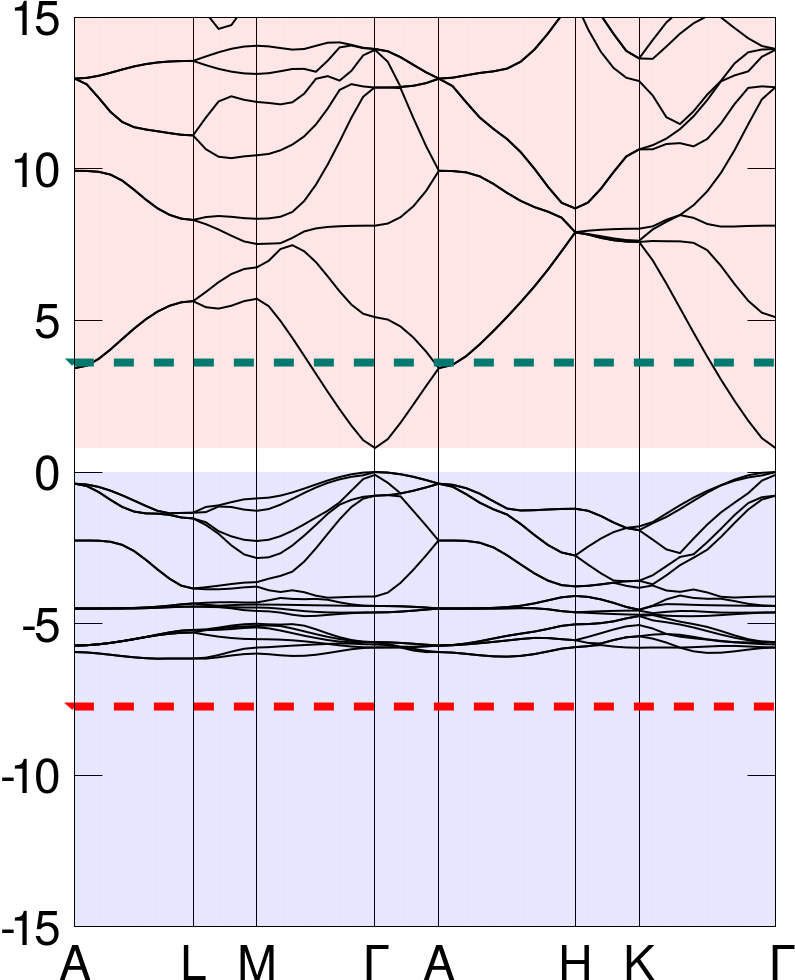
\includegraphics[width=0.35\textwidth]{../figures/ZnO_lda.png}};
                        \node[font=\tiny,color=exp_green] (exp label) at (2.5,2) {exp.};
                        \node[above,align=center,font=\small] at (dft.north) {DFT systematically\\underestimates\\the band gap};
                        \node[inner sep=0pt] (koopmans) at (18,0)
                        {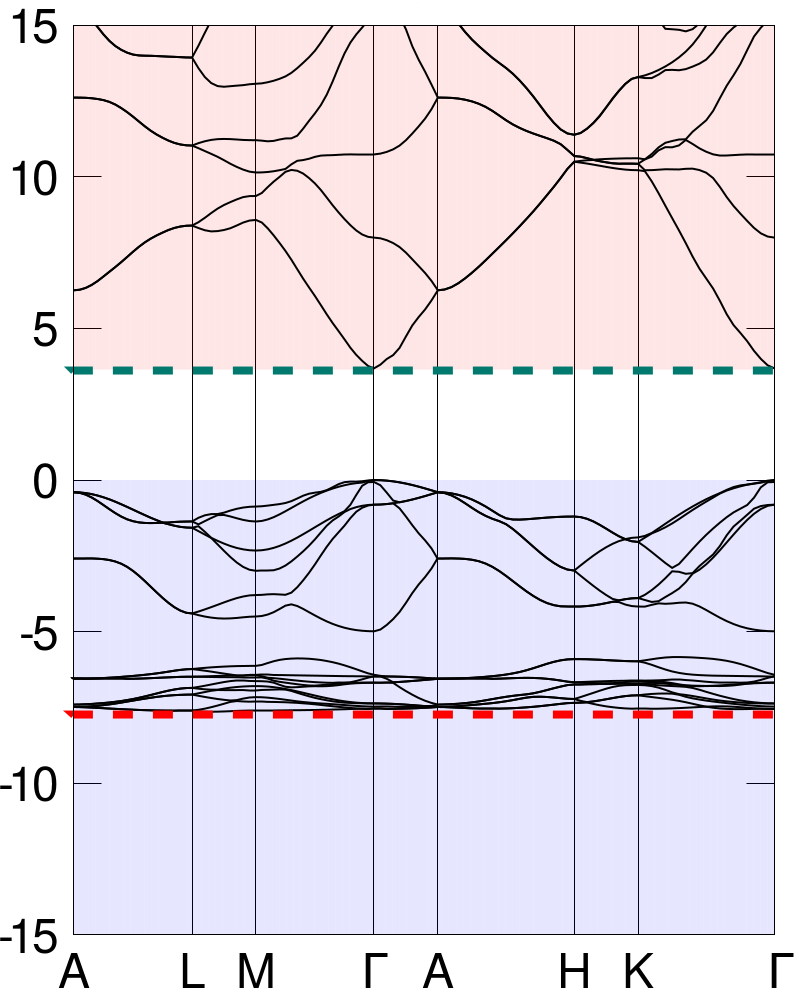
\includegraphics[width=0.35\textwidth]{../figures/ZnO_ki.png}};
                        \node[above,align=center,font=\small] at (koopmans.north) {Koopmans\\accurately predicts\\the band gap};
                        \node[align=center, font=\scriptsize] (midpoint) at (9,2) {impose generalised\\piecewise linearity};
                        \draw[shorten <= 0.5cm, line width=0.15cm] ([yshift=-1cm] dft.east) to[out=45, in=180] (midpoint.south);
                        \draw[shorten >= 0.5cm, line width=0.15cm, -{Latex[round,width=0.75cm,length=1cm]}] (midpoint.south) to[out=0, in=135] ([yshift=-1cm] koopmans.west);
                    \end{tikzpicture}
                    \end{center}

                    \setlength{\tabcolsep}{5pt}
                    \renewcommand{\arraystretch}{1}

                    \vspace{1ex}
                    \hbox{
                    \begin{minipage}{0.5\columnwidth}
                    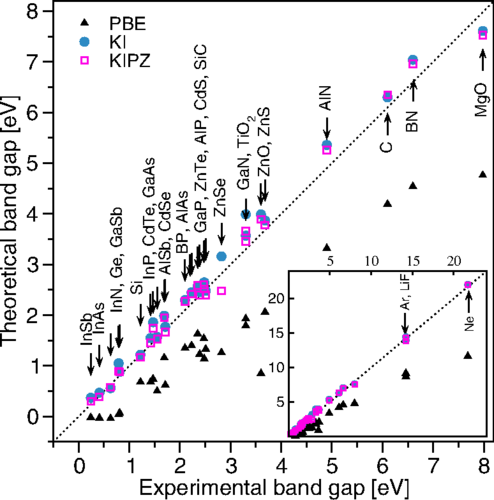
\includegraphics[width=\columnwidth,valign=t]{../figures/nguyen2018_bandgaps.png}

                    \scriptsize
                    \begin{tabular}{c c S[table-format = 2.2] S[table-format = 2.2] S[table-format = 2.2] S[table-format = 2.2] S[table-format = 2.2] S[table-format = 2.2] S[table-format = 2.2] S[table-format = 2.2] S[table-format = 2.2]}
                                                          &             & {PBE} & {G\textsubscript{0}W\textsubscript{0}} & {KI} & {KIPZ} & {QSG$\tilde{\mathrm{W}}$} \\
                        \midrule
                        \midrule
                        \multirow{2}{*}{$E_\mathrm{gap}$} &
                        {MAE (eV)}                        & 2.54        & 0.56  & 0.27                                   & 0.22 & 0.18                               \\
                                                          & {MAPE (\%)} & 48.28 & 12.10                                  & 7.09 & 5.37   & 4.46                      \\
                        \midrule
                        \multirow{2}{*}{IP}               &
                        {MAE (eV)}                        & 1.09        & 0.39  & 0.19                                   & 0.21 & 0.49                               \\
                                                          & {MAPE (\%)} & 15.58 & 5.71                                   & 2.99 & 3.14   & 7.41
                    \end{tabular}
                        
                    \end{minipage}
                    \hspace{0.05\columnwidth}
                    \begin{minipage}{0.4\columnwidth}
                        \raggedright
                    \textbf{Semiconductors and insulators} Band gap and ionisation potential of semiconductors and insulators compared to experiment
                    
                    \textcolor{kgrey_light}{\citeauthoryear{Nguyen2018}}
                    \end{minipage}
                    }

                    \vspace{1em}
                    \normalsize

                    \textbf{Molecules} The KI, pKIPZ, and KIPZ Koopmans functionals give ionization potentials comparable to state-of-the-art GW across the GW100 dataset
                    
                    \textcolor{kgrey_light}{\citeauthoryear{Colonna2019}}

                    \vspace{0.5em}

                    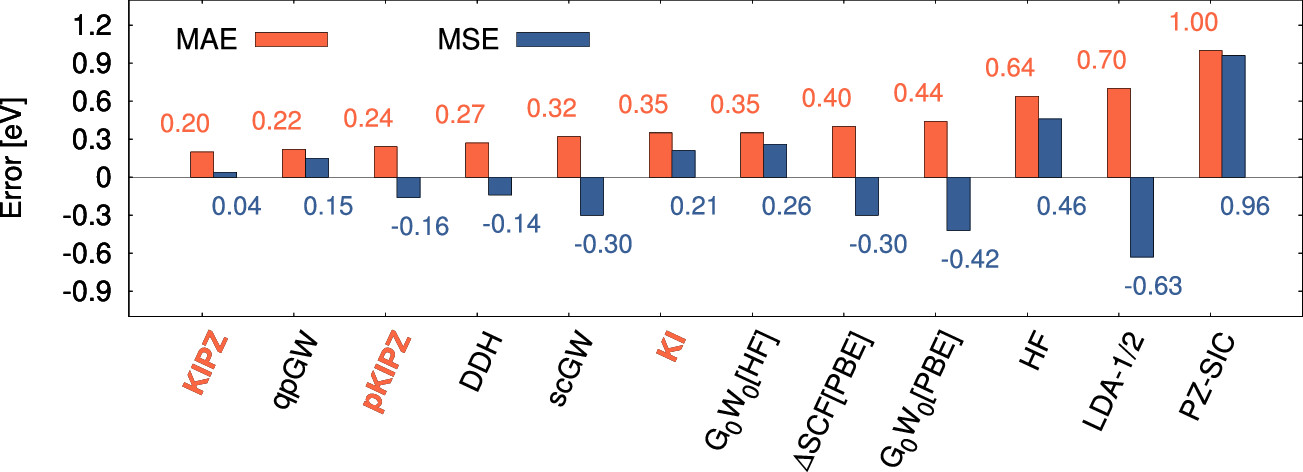
\includegraphics[width=0.9\columnwidth]{../figures/colonna_2019_gw100_ip.jpeg}

                    \vspace{0.15em}

                \end{block}

            \end{column}

            \begin{column}{0.57\linewidth}

                \begin{block}{2. How do Koopmans functionals work?}
                    \nocite{Dabo2009,Dabo2010,Borghi2014,Colonna2018,Nguyen2018,Colonna2019,DeGennaro2022,Colonna2022,Linscott2023}
                    Koopmans functionals are constructed to reproduce spectral properties (charged excitations) and total energies on the same footing, enforcing a generalised piecewise linearity condition.
                    \vspace{0.125em}
                    \begin{equation*}
                        E_\mathrm{Koopmans} = E_\mathrm{DFT} + \sum_i \alpha_i \biggl( \underbrace{- \int_0^{f_i}\varepsilon_i(f) df}_{\substack{\text{removes the erroneous} \\ \text{curvature}}} \underbrace{+ f_i\int_0^1 \varepsilon_i(f) df}_{\substack{\text{restores the}\\ \text{correct linearity}}} \biggr)
                    \end{equation*}
                    \vspace{0.125em}

                    As the results on the left show, this strategy is sufficient to obtain band structures and orbital energies as accurate as state-of-the-art GW, at a fraction of the computational cost.

                    \vspace{1ex}
                    However, there's no such thing as a free lunch: compared to DFT these calculations are require a few extra steps:
                    \begin{itemize}
                        \item obtaining a set of localized orbitals $\rightarrow$ the focus of this work
                        \item calculating screening parameters $\rightarrow$ implemented and automated in the \texttt{koopmans} code \textcolor{kgrey_light}{\citeauthoryear{Linscott2023}}
                    \end{itemize}

                    \vspace{0.34em}
                \end{block}

                \vspace{1.5ex}

            \begin{block}{3. Localized orbitals via automated Wannierization}
                In order to automate the Wannierisation, we...

                \vspace{1ex}
                \begin{columns}
                    \begin{column}{0.35\columnwidth}
                \textbf{(a) use pseudoatomic orbitals as projectors}

                \begin{tikzpicture}
                    \node[font=\tt\small,align=left] (old) at (0,0) {begin projections\\\qquad f=0.25,0.25,0.25:sp3\\end projections};
                    \draw[color=seaborn_red, line width=0.1cm] (old.south west) -- (old.north east);
                    \draw[color=seaborn_red, line width=0.1cm] (old.north west) -- (old.south east);
                \end{tikzpicture}

                \vspace{1ex}
                \textbf{(b) perform disentanglement based on projectability}

                \begin{center}
                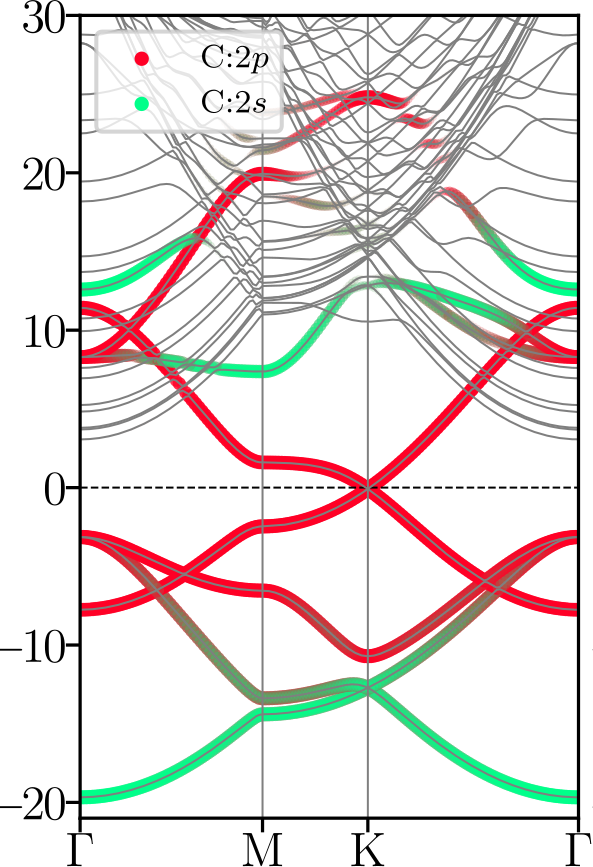
\includegraphics[width=0.6\columnwidth]{../figures/proj_disentanglement_fig1a.png}
                \end{center}

                System-dependent energy disentanglement windows are no longer required
                \textcolor{kgrey_light}{\citeauthoryear{Qiao2023}}
                        
                    \end{column}
                    \begin{column}{0.5\columnwidth}
                \textbf{(c) separate subspaces via parallel transport}
                
                \begin{center}
                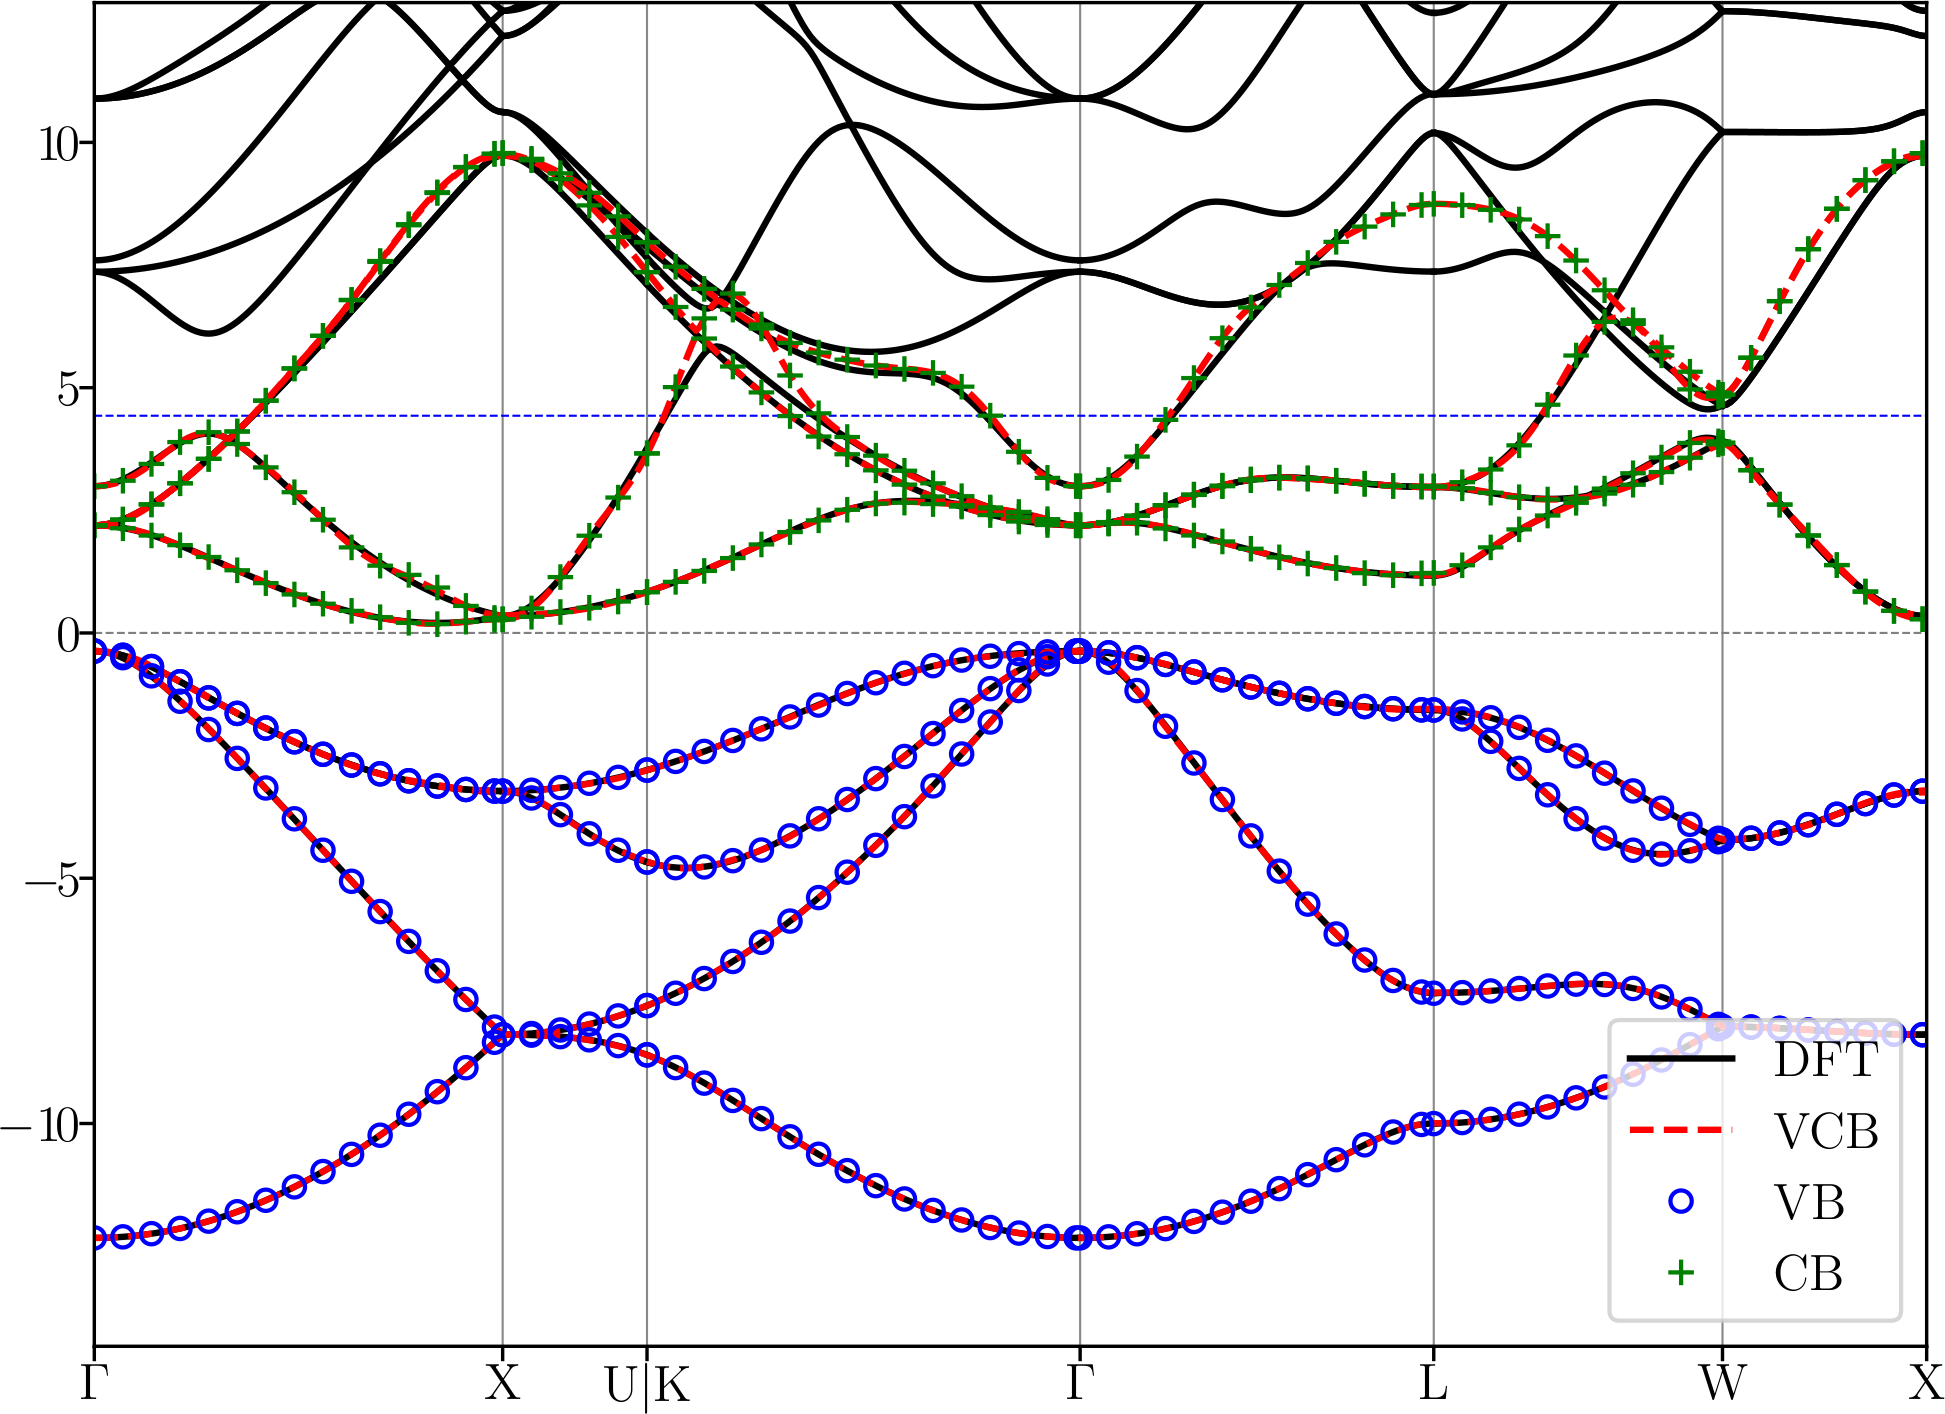
\includegraphics[width=0.6\columnwidth]{../figures/target_manifolds_fig1b.png}
                \end{center}

                \textcolor{kgrey_light}{\citeauthoryear{Qiao2023a}}
                \vspace{1ex}

                \textbf{(d) extend the pseudoatomic orbital basis}

                \vspace{1ex}
                \begin{center}
                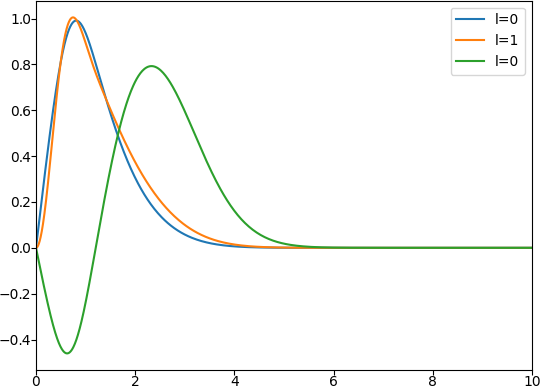
\includegraphics[width=0.6\columnwidth]{../paos/F_with_3s_cropped.png}
                \end{center}

                Requires a confining potential for higher states, which is parametrised via Bayesian optimisation
                        
                    \end{column}
                \end{columns}



            \end{block}

            \end{column}

        \end{columns}

        % \vspace{1em}
        % \begin{columns}
        %     \begin{column}{0.968\textwidth}
        %         \begin{block}{3. Workflows}
        %             \vspace{1ex}
        %             \begin{center}
        %                 \begin{minipage}{0.85\textwidth}
        %                     Supercell implementation

        %                     \vspace{-3ex}
        %                     \begin{tikzpicture}[font=\tiny, x=6cm, y=2cm]
   \begin{pgfonlayer}{background}
      % \node[fit= (KC init) (empty label) (filled label) (sc loop 1) (converged label), fill=seaborn_bg_grey, inner sep=0.5cm] (calculating screening) {};
      % \node [dummy, above=0cm of calculating screening, font=\sffamily]{Calculating screening parameters};
      \fill [seaborn_bg_grey] (-2.1,-0.8) rectangle (1.3,4.6);
      \node at (-2.1, 4.6) [default_text, font=\footnotesize] {Initialisation (molecules)};
      \fill [seaborn_bg_grey] (-2.1,-4.6) rectangle (1.3,-1.2);
      \node at (-2.1, -1.2) [default_text, font=\footnotesize] {Initialisation (solids)};
      \fill [seaborn_bg_grey] (1.4,-4.6) rectangle (6.9,4.6);
      \node at (1.4, 4.6) [default_text, font=\footnotesize, text width=4.5cm] {Calculating screening parameters};
      \fill [seaborn_bg_grey] (7,-4.6) rectangle (8,4.6);
      \node at (7, 4.6) [default_text, font=\footnotesize, text width=6cm] {Final calculation};
      \fill [seaborn_bg_grey] (8.1,-4.6) rectangle (9.1,4.6);
      \node at (8.1, 4.6) [default_text, font=\footnotesize, text width=6cm] {Postprocessing (solids)};
   \end{pgfonlayer}

   % Key
   \node at (5.84, 5.25) [cp, text width=2.4cm, minimum height=1.7cm, font=\tiny] {\texttt{kcp}};
   \node at (6.44, 5.25) [kcw, text width=2.4cm, minimum height=1.7cm, font=\tiny] {\texttt{kcw}};
   \node at (7.04, 5.25) [pw, text width=2.4cm, minimum height=1.7cm, font=\tiny] {\texttt{pw}};
   \node at (7.64, 5.25) [wannier90, text width=2.4cm, minimum height=1.7cm, font=\tiny] {\texttt{wannier}};
   \node at (8.24, 5.25) [bespoke, text width=2.4cm, minimum height=1.7cm, font=\tiny] {bespoke code};
   \node at (8.84, 5.25) [observable, text width=2.4cm, minimum height=1.7cm, font=\tiny] {quantity of interest};

   % Initialisation
   % Option 1
   \node at (-1, 2.9) [cp] (DFT init) {DFT};
   \node at (0, 2.9) [cp] (PZ innerloop) {PZ unitary rotation};
   \path [line] (DFT init) -- (PZ innerloop);

   % OR
   \node at (-0.5, 1.9) [default] (or) {or};

   % Option 2
   \node at (-0.5, 0.9) [cp] (PZ init) {PZ};

   % Solids
   \node at (-1.5, -2.9) [pw] (pw DFT init) {DFT (primitive cell)};
   \node at (-0.5, -2.9) [wannier90] (wannierize) {wannierize};
   \node at (0.5, -2.9) [bespoke] (unfold) {fold to supercell};
   \path [line] (pw DFT init) -- (wannierize);
   \path [line] (wannierize) -- (unfold);

   % Calculating screening parameters
   \node at (2, 0) [cp] (KC init) {$\alpha_0$KI/$\alpha_0$KIPZ};

   \path let
   \p1 = (PZ innerloop),
   \p2 = (unfold.east)
   in
   coordinate (dummy) at (\x2, \y1);
   \path let
   \p1 = (PZ init),
   \p2 = (unfold.east)
   in
   coordinate (dummy2) at (\x2, \y1);
   \path [line] (PZ innerloop) -- (dummy) to[-|-=0.3] ([yshift=2\myyshift]KC init.west);
   \path [line] (PZ init.east) -- ([xshift=-3.5\myyshift]dummy2) to[-|-=0.3] (KC init.west);
   \path [line] ([yshift=-2\myyshift]unfold.east) to[-|-=0.3] ([yshift=-2\myyshift]KC init.west);

   % KI filled %%%%%%%%%%%%%%%%%%%%%%%%%%%%%%%%%%%%%%%%%%%%%%%%%%

   % calculations
   \node at (3, 3) [cp] (N-1_filled) {DFT/$\alpha_0$KIPZ ($N-1$)};
   \node at (3, 2) [cp] (DFT_filled) {DFT};
   \node at (3, -2) [cp] (DFT_empty) {DFT};
   \node at (3, -3) [cp] (N+1_empty) {DFT/$\alpha_0$KIPZ ($N+1$)};

   \path [line] (KC init) to[-|-] (DFT_filled);
   \path [line] (KC init) to[-|-] (N-1_filled);
   \path [line] (KC init) to[-|-] (DFT_empty);
   \path [line] (KC init) to[-|-] (N+1_empty);

   % results
   \node at (4, 3) [observable] (EN-1_filled) {$E_i(N-1)$};
   \node at (4, 2) [observable] (lambda0_filled) {$\lambda^{0}_{ii}(1)$};
   \node at (4, 1) [observable] (lambda_filled) {$\lambda^{\alpha_0}_{ii}(1)$};
   \node at (4, 0) [observable] (EN) {$E(N)$};
   \node at (4, -1) [observable] (lambda_empty) {$\lambda^{\alpha_0}_{ii}(0)$};
   \node at (4, -2) [observable] (lambda0_empty) {$\lambda^{0}_{ii}(0)$};
   \node at (4, -3) [observable] (EN+1_empty) {$E_i(N+1)$};

   \path [line] (KC init) -- (EN);
   \path [line] (KC init.east) to[-|-] (lambda_filled.west);
   \path [line] (KC init.east) to[-|-] (lambda_empty.west);

   \path [line] (DFT_filled) -- (lambda0_filled);
   \path [line] (N-1_filled) -- (EN-1_filled);

   \path [line] (DFT_empty) -- (lambda0_empty);
   \path [line] (N+1_empty) -- (EN+1_empty);

   % alpha parameters
   \node at (5, 1.5) [observable] (alpha filled) {$\alpha_{i \in \text{filled}}$};
   \node at (5, -1.5) [observable] (alpha empty) {$\alpha_{i \in \text{empty}}$};

   \path [line] (lambda_filled) to[-|-] (alpha filled);
   \path [line] ([yshift=\myyshift]EN.east) to[-|-] (alpha filled.west);
   \path [line] (lambda0_filled) to[-|-] (alpha filled);
   \path [line] (EN-1_filled) to[-|-] (alpha filled);

   \path [line] (lambda_empty) to[-|-] (alpha empty);
   \path [line] ([yshift=-\myyshift]EN.east) to[-|-] (alpha empty.west);
   \path [line] (lambda0_empty) to[-|-] (alpha empty);
   \path [line] (EN+1_empty) to[-|-] (alpha empty);

   % SC check
   \coordinate (sc check) at (6, 0);
   \path [headless_line] (alpha empty) to[-|-] (sc check);
   \path [headless_line] (alpha filled) to[-|-] (sc check);

   % Final calc
   \node at (7.5, 0) [cp] (final KI) {$\alpha$KI/$\alpha$KIPZ};
   \path [line] (sc check) -- node [midway, above, font=\sffamily\tiny] (converged label) {$\{\alpha_i\}$ converged} (final KI);

   % Postproc
   \node at (8.6, 0) [bespoke] (upfold) {unfold to primitive cell};
   \path [line] (final KI) -- (upfold);

   % Boxes
   % Screening parametere
   \node [boxwhite, fit= (N-1_filled) (lambda_filled) (alpha filled),
      draw, dashed, fill opacity=0, inner sep=0.45cm](filled box){};
   \node [dummy, above=0cm of filled box, font=\sffamily](filled label){\tiny one per unique filled orbital (index $i$)};
   \node [boxwhite, fit= (N+1_empty) (lambda_empty) (alpha empty),
      draw, dashed, fill opacity=0, inner sep=0.45cm](empty box){};
   \node [dummy, below=0cm of empty box, font=\sffamily](empty label){\tiny one per unique empty orbital (index $i$)};

   % SC loop
   \node [below=-0.4cm of empty label] (sc loop y) {};
   \path let
   \p1 = (sc check),
   \p2 = (sc loop y)
   in
   coordinate (sc loop 1) at (\x1, \y2);
   \path [line] (sc check) -- node [midway, right, font=\sffamily\tiny, align=left] (not converged label) {$\{\alpha_i\}$ not\\converged} (sc loop 1) -| (KC init.south);


   % \onslide<2->{
   %    \node at (3.5, 0) [default_text, fill=white, opacity=0.9, text opacity=1, anchor=center, minimum height=5cm, text width=7.5cm, execute at begin node=\setlength{\baselineskip}{30pt}] (nc text) {
   %       \huge Riccardo De Gennaro
   %       \textbf{M22.00004} / paper in preparation
   %    };
   %    \node[right = -0.2cm of nc text, anchor=west]{\includegraphics[height=5cm]{figures/riccardo_degennaro.jpg}};
   % }

\end{tikzpicture}


        %                     \vspace{-2ex}
        %                     \noindent Primitive cell implementation

        %                     \vspace{0.5ex}
        %                     \begin{tikzpicture}[font=\tiny, x=6cm, y=2cm]
   \begin{pgfonlayer}{background}
      \fill [seaborn_bg_grey] (-2.2,-1) rectangle (1.2,1.5);
      \node at (-2.2, 1.5) [default_text] {\footnotesize Initialisation};
      \fill [seaborn_bg_grey] (1.3,-1) rectangle (3.7,1.5);
      \node at (1.3, 1.5) [default_text] {\footnotesize Calculating screening parameters};
      \fill [seaborn_bg_grey] (3.8,-1) rectangle (5.2,1.5);
      \node at (3.8, 1.5) [default_text, text width=7cm] {\footnotesize Final calculation};
      % \fill [seaborn_bg_grey] (8.1,-1) rectangle (9.1,1.5);
      % \node at (8.1, 1.5) [default_text, text width=3.5cm] {\large Postprocessing};
   \end{pgfonlayer}

   % % Key
   % \node at (3.45, 2.15) [pw, text width=1.4cm, minimum height=0.7cm] {\texttt{pw}};
   % \node at (3.95, 2.15) [wannier90, text width=1.4cm, minimum height=0.7cm] {\texttt{wannier90}};
   % \node at (4.45, 2.15) [bespoke, text width=1.4cm, minimum height=0.7cm, font=\tiny] {bespoke code};
   % \node at (4.95, 2.15) [observable, text width=1.4cm, minimum height=0.7cm, font=\tiny] {quantity of interest};

   % Initialisation
   % Solids
   \node at (-1.5, 0) [pw] (pw DFT init) {DFT};
   \node at (-0.5, 0) [wannier90] (wannierize) {wannierize};
   \node at (0.5, 0) [observable] (unfold) {$\{\ket{w_i}\}$};
   \path [line] (pw DFT init) -- (wannierize);
   \path [line] (wannierize) -- (unfold);

   % Calculating screening parameters
   \node at (2, 0) [kcw] (KC screen) {DFPT calculation};
   \node at (3, 0) [observable] (alphas) {$\{\alpha_i\}$};
   \path [line] (unfold) -- (KC screen);
   \path [line] (KC screen) -- (alphas);

   % Final calc
   \node at (4.5, 0) [kcw] (KC ham) {$\alpha_0$KI/$\alpha_0$KIPZ};
   \path [line] (alphas) -- (KC ham);

   % \onslide<4->{
   %    \node at (1, 0) [default_text, fill=white, opacity=0.9, text opacity=1, anchor=center, minimum height=5cm, text width=7cm, execute at begin node=\setlength{\baselineskip}{30pt}] (nc text) {
   %       \huge Nicola Colonna
   %       \textbf{A20.00002} /
   %       paper in preparation
   %    };
   %    \node[right = -0.2cm of nc text, anchor=west]{\includegraphics[height=5cm]{figures/nicola_colonna.png}};
   % }

\end{tikzpicture}

        %                 \end{minipage}
        %             \end{center}
        %         \end{block}
        %     \end{column}
        % \end{columns}

        \vspace{1.4ex}
        \begin{columns}[t]
            \begin{column}{0.67\textwidth}
                \begin{block}{References\vphantom{g}}
                    \vspace{0.4em}
                    \hspace{-2em}
                    \begin{minipage}{1.03\textwidth}
                        \AtNextBibliography{\tiny}
                        \printbibliography
                    \end{minipage}
                \end{block}

            \end{column}

            \begin{column}{0.27\textwidth}
                % \setbeamercolor{block title}{bg=white, fg=white}
                % \begin{block}{\vphantom{P}}
                %     \vspace{-2.8ex}
                %     or run with \texttt{python}:
                %     \inputminted[fontsize=\tiny, autogobble, breaklines]{python}{scripts/si.py}
                % \end{block}

                % \vspace{1em}
                % \setbeamercolor{block title}{bg=kgrey, fg=white}
                \begin{block}{Acknowledgements}
                    \vspace{0.5em}
                    
\includegraphics[height=0.1\columnwidth]{../figures/psi_trimmed.png}
                    \hfill
                    
\includegraphics[height=0.1\columnwidth]{../figures/marvel_trimmed.png}
                    \hfill
                    
\includegraphics[height=0.1\columnwidth]{../figures/SNF_logo_standard_print_color_pos_e.eps}
                    \vspace{0.5em}

                    \footnotesize
                    This work was supported by the Swiss National Science
                    Foundation (SNSF) through its National Centre of Competence in Research (NCCR) MARVEL and Grant No.
                    200021-179138. The National Centres of Competence in Research (NCCRs) are a funding scheme of the Swiss National Science Foundation
                    \vspace{0.5em}


                \end{block}
                % \begin{beamercolorbox}[wd=\textwidth,sep=1em]{logos}
                % \end{beamercolorbox}

            \end{column}
        \end{columns}

        \vspace{1.4ex}

    \end{beamercolorbox}

    \setbeamercolor{banner}{fg=white,bg=kgrey}
    \begin{beamercolorbox}[wd=\textwidth,sep=1em]{banner}
        \begin{center}
            \bf \large Go to {\ttfamily \bf \large koopmans-functionals.org} to find out more!
        \end{center}
        \vspace{0.005\paperheight}
    \end{beamercolorbox}

\end{frame}
% \setlength{\myimscale}{0.08\textwidth}
% \begin{tikzpicture}[every node/.style={color=kgrey}]
%     \node[inner sep=0pt] (logo) at (3\myimscale,0\myimscale)
%     {
\includegraphics[width=0.7\textwidth]{figures/k_grey_on_transparent.png}};
%     \node[rectangle, draw, thick, minimum width=5.75\myimscale, minimum height=3.5\myimscale, outer sep=0, label=above:linearisation,
%         path picture={
%                 \node at (path picture bounding box.center){
%                     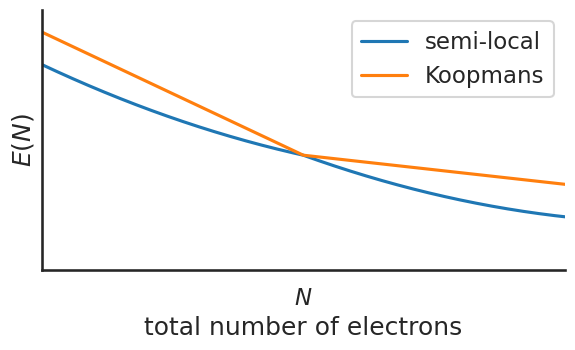
\includegraphics[width=5.75\myimscale]{figures/linearisation.png}
%                 };
%             }] (linear) at (0\myimscale,5.2\myimscale) {};
%     \node[rectangle, draw, thick, minimum width=5.75\myimscale, minimum height=3.5\myimscale, outer sep=0, label=above:screening,
%         path picture={
%                 \node at (path picture bounding box.center){
%                     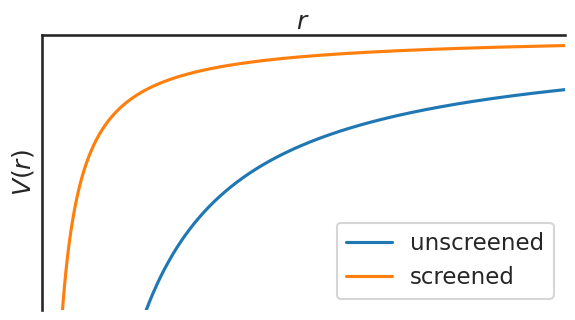
\includegraphics[width=5.75\myimscale]{figures/screening.png}
%                 };
%             }] (screening) at (6.25\myimscale,5.2\myimscale) {};
%     \node[rectangle, minimum width=2.5\myimscale, minimum height=3.5\myimscale, outer sep=0,
%         path picture={
%                 \node at ([yshift=-0.05\myimscale]path picture bounding box.center){
%                     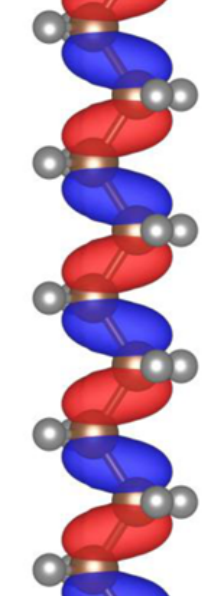
\includegraphics[width=2.5\myimscale]{figures/fig_nguyen_canonical_orbital.png}
%                 };
%             }] (bloch) at (-1.5\myimscale,-5.2\myimscale) {};
%     \node[rectangle, minimum width=2.5\myimscale, minimum height=3.5\myimscale, outer sep=0,
%         path picture={
%                 \node at ([yshift=1.5\myimscale]path picture bounding box.center){
%                     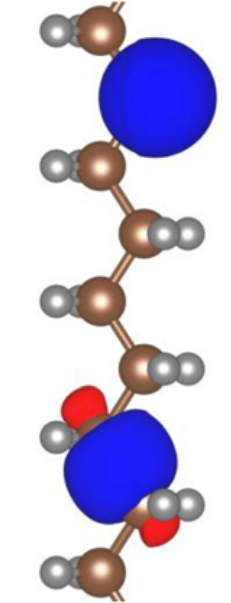
\includegraphics[width=2.6\myimscale]{figures/fig_nguyen_variational_orbital.png}
%                 };
%             }] (wannier) at (1.5\myimscale,-5.2\myimscale) {};
%     \node[rectangle, draw, thick, minimum width=5.75\myimscale, minimum height=3.5\myimscale, outer sep=0, label=below:localisation,
%     ] (localisation) at (0\myimscale,-5.2\myimscale) {};
%     \node[rectangle, draw, thick, minimum width=5.75\myimscale, minimum height=3.5\myimscale, outer sep=0, label=below:automation,
%         path picture={
%                 \node at (path picture bounding box.east){
%                     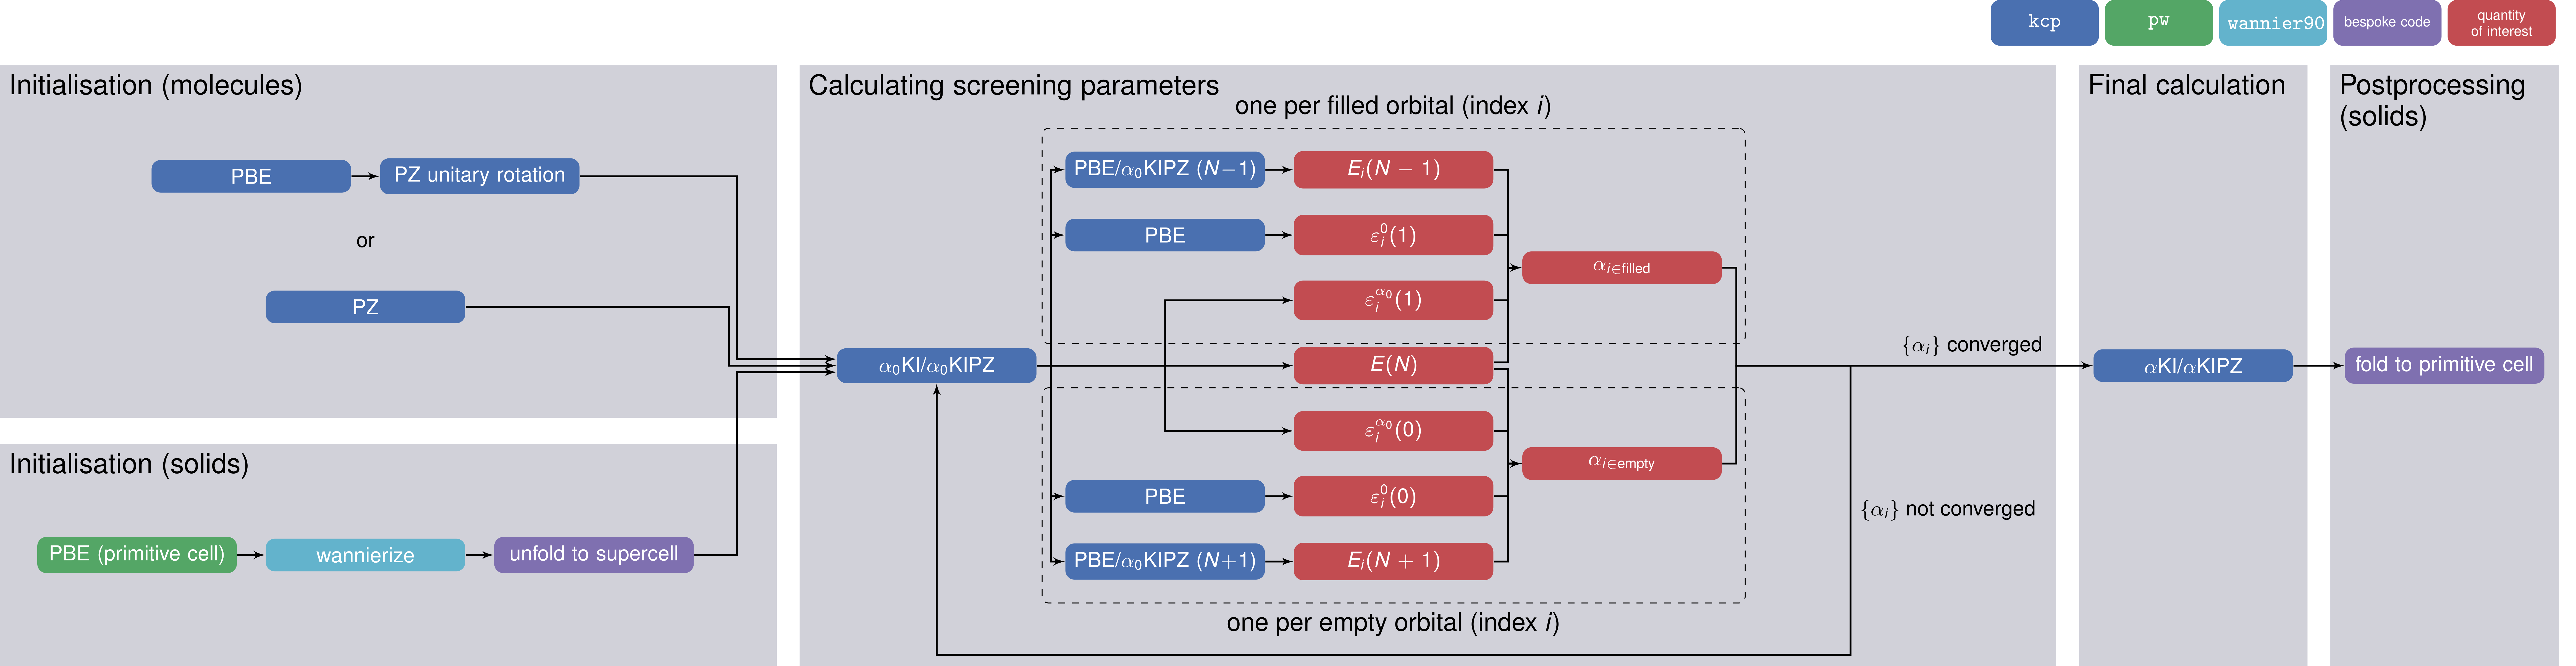
\includegraphics[width=15\myimscale]{figures/dscf_workflow.png}
%                 };
%             }] (workflow) at (6.25\myimscale,-5.2\myimscale) {};
%     \draw[thick, -{Latex[round]}] (bloch) -- (wannier);
% \end{tikzpicture}

\end{document}
